\documentclass[sigconf]{acmart}
% Local preview support; replace with the organizer's preamble when available.
\newif\ifguideStyle
\newcommand{\guide}[1]{%
  \ifguideStyle
    {\color{gray!65}\itshape #1}%
  \fi
}

\guideStylefalse
\setcopyright{none}
\settopmatter{printacmref=false}
\acmConference[Technical Report]{Competition Technical Report}{November 2026}{Online}
\acmYear{2026}
\acmDOI{}
\acmISBN{}
\setlength{\emergencystretch}{1em}
\setcounter{dbltopnumber}{3}
\renewcommand{\dbltopfraction}{0.99}
\renewcommand{\textfraction}{0.01}
\setlength{\dblfloatsep}{5pt}
\setlength{\dbltextfloatsep}{7pt}
\setlength{\textfloatsep}{7pt}

\begin{document}
\title{Solar Filament Instance Segmentation in H-Alpha Images}
\subtitle{Final Technical Report: Five Scored Pipelines}
\author{Gregory Kojadinovich II}
\affiliation{%
  \institution{Europa Waters LLC}
  \city{South Lake Tahoe, CA}
  \country{USA}
}
\email{gregkoja3343@icloud.com}

\begin{abstract}
I evaluate five pipelines for solar filament instance segmentation.
Public panoptic quality (PQ) is 0.29 and 0.32 for semantic U-Net baselines,
0.35 for YOLO with crop refinement, and 0.36 for a five-fold
YOLO/ResNet34-U-Net pipeline. A five-fold YOLO-only follow-up, allowing
10 detector epochs per fold without a training deadline, scores 0.26.
The results favor retaining crop refinement as a candidate stage rather
than relying on a larger detector epoch allowance. However, training,
calibration, and other settings also differ; the 0.10 PQ gap is not an
isolated measurement of cropping's effect.
\end{abstract}

\begin{teaserfigure}
\centering
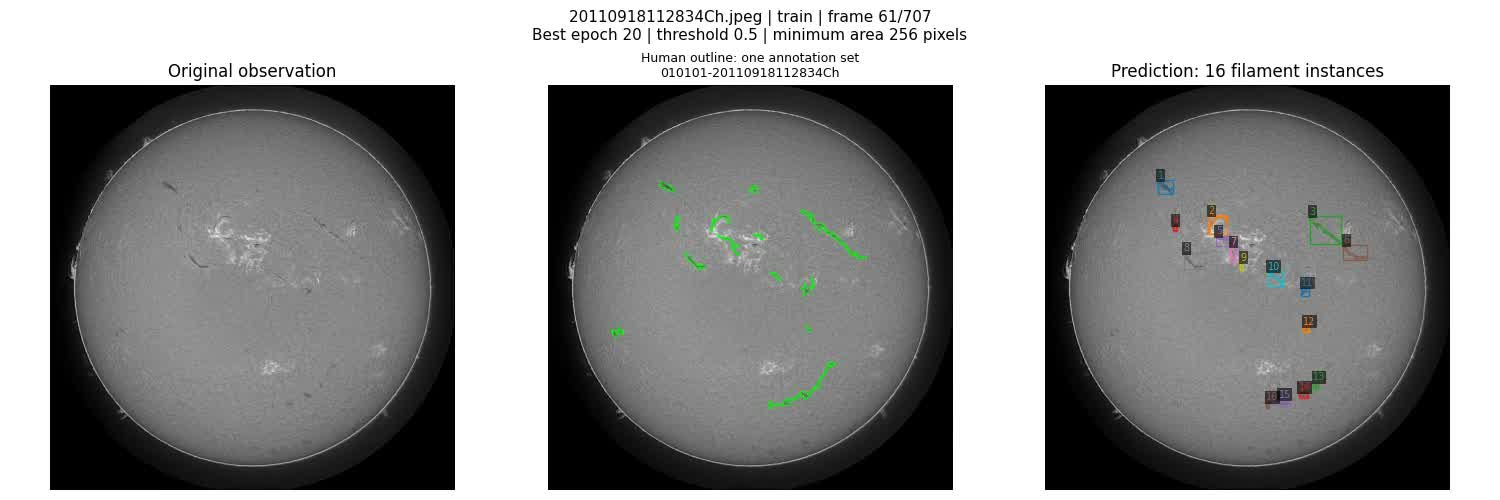
\includegraphics[width=0.80\textwidth]{../Baseline Video/thumbnail.jpg}
\caption{Baseline review frame: observation, annotation, and model overlay.
The sequence includes training images and is qualitative, not independent
evaluation.}
\label{fig:baseline}
\end{teaserfigure}
\maketitle

\begin{figure*}[t]
\centering
\large
\begin{tabular}{ccccc}
\shortstack{0.29\\\textcolor{blue!65!black}{\rule{1.1cm}{14.5mm}}\\V1} &
\shortstack{0.32\\\textcolor{orange!85!black}{\rule{1.1cm}{16mm}}\\V2} &
\shortstack{0.35\\\textcolor{green!50!black}{\rule{1.1cm}{17.5mm}}\\V3} &
\shortstack{0.36\\\textcolor{purple!70!black}{\rule{1.1cm}{18mm}}\\V5} &
\shortstack{0.26\\\textcolor{red!65!black}{\rule{1.1cm}{13mm}}\\V7}
\end{tabular}

\smallskip
\normalsize
\begin{tabular}{llll}
\hline
Run & Main model & Image size & Crop refiner \\
\hline
V1 & ResNet18 U-Net & 512 px & None \\
V2 & ResNet18 U-Net & 1024 px & None \\
V3 & YOLO11s-seg & 1024 px & ResNet18 U-Net, 256 px \\
V5 & 5 $\times$ YOLO11s-seg & 1024 px & ResNet34 U-Net, fold-selected \\
V7 & 5 $\times$ YOLO11s-seg & 1024 px & None \\
\hline
\end{tabular}
\caption{Verified public PQ and pipeline configurations. V7 scores 0.10
below V5 and 0.09 below V3. These are whole-pipeline comparisons.}
\label{fig:scores}
\end{figure*}

\section{Context and Evaluation}
The challenge uses grayscale GONG H-$\alpha$ intensity images and
annotator-specific filament masks~\cite{filament-segmentation-2026,ahmadzadeh2024dataset}.
The data comprise 707 labeled photographs, 1,154 annotator image sets,
8,199 instances, and 180 unlabeled test images. V1--V3 use a fixed
day-grouped split of 499 training, 103 tuning, and 105 holdout photographs
(seed 2026). All annotation sets for a photograph remain together.
Local metrics average annotators within photographs, then photographs.

The ESAIR poster addresses boundaries, grouping, and
chirality~\cite{esairposter2026}. H-Alpha Anomalyzer and an anomaly-detection
review provide observation-quality context~\cite{khazaei2025software,khazaei2025icdm,ruff2021anomaly};
their methods are not implemented here. Two public U-Net notebooks were
reviewed~\cite{pavlonotebook,foysalnotebook}; the independently written V3
detector/refiner design was informed by the YOLO/U-Net
notebook~\cite{ektarrnotebook}. No score parity is claimed.

Panoptic quality measures recognition and overlap~\cite{pq}:
\begin{equation}
\mathrm{PQ}=
\frac{\sum_{(p,g)\in TP}\mathrm{IoU}(p,g)}
{|TP|+\tfrac12|FP|+\tfrac12|FN|}.
\end{equation}
Local instance matching requires IoU strictly greater than 0.5.
The public scores are single-run measurements without repeated-seed
uncertainty; foreground overlap and CSV validity do not substitute for PQ.

\begin{figure*}[t]
\centering
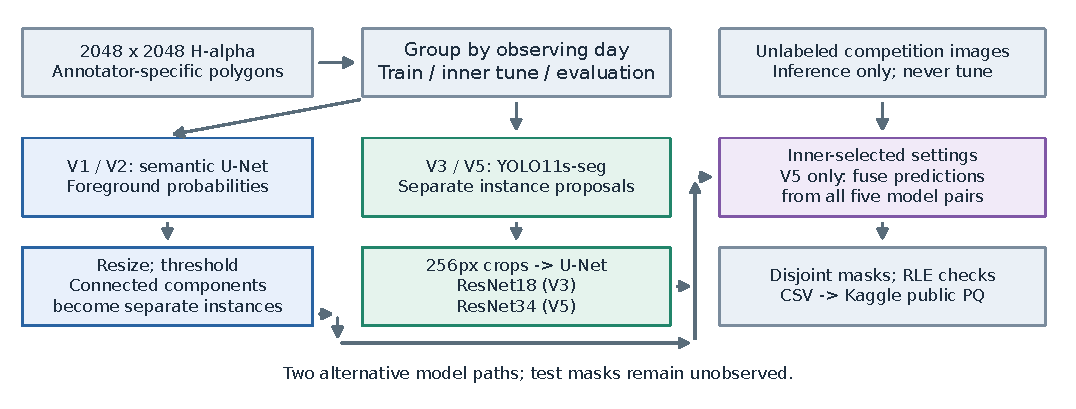
\includegraphics[width=0.75\textwidth]{figures-v2/workflow.pdf}
\caption{Semantic and instance-aware pipelines. Crop refinement is a local
prediction stage, not a crop of the competition's evaluation area.}
\label{fig:workflow}
\end{figure*}

\begin{figure*}[t]
\centering
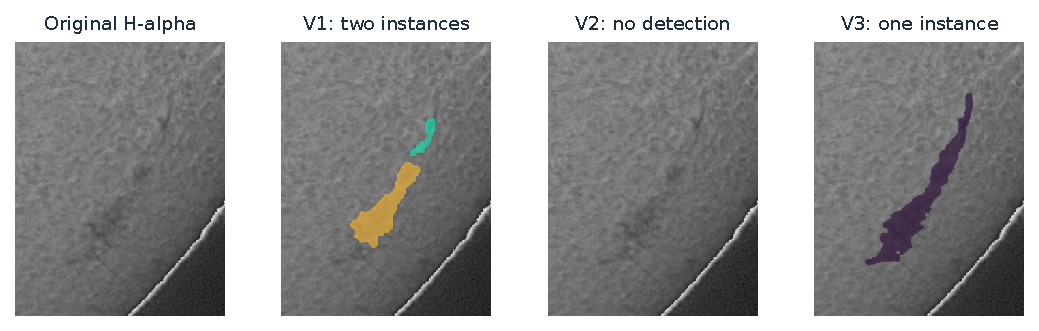
\includegraphics[width=0.75\textwidth]{figures-v2/mask_comparison.pdf}
\caption{V1--V3 predictions for a disagreement-selected test crop:
\texttt{20210708060030Lh.jpeg}, $x=[1502,1767)$, $y=[1328,1673)$.
Colors identify instances, not correctness. This panel does not depict V7.}
\label{fig:masks}
\end{figure*}

\begin{figure*}[t]
\centering
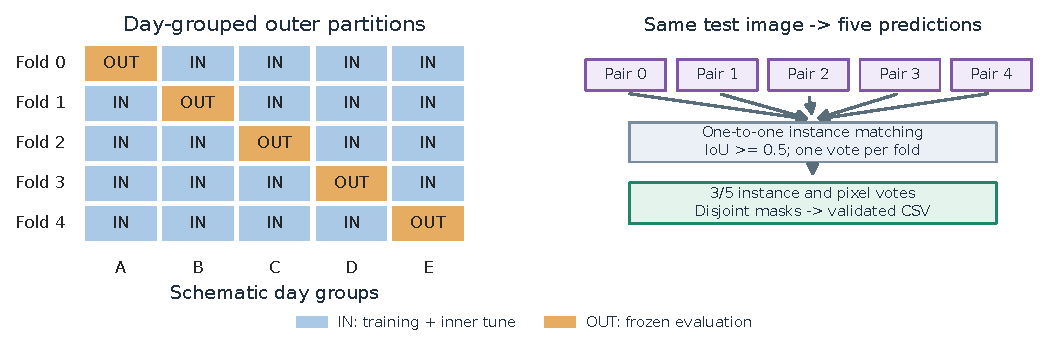
\includegraphics[width=0.75\textwidth]{figures-v2/folds_and_fusion.pdf}
\caption{Day-grouped folds and five-model fusion. IN includes training and
inner tuning; OUT is held out. Each instance and pixel requires three votes.}
\label{fig:folds}
\end{figure*}

\begin{figure*}[t]
\centering
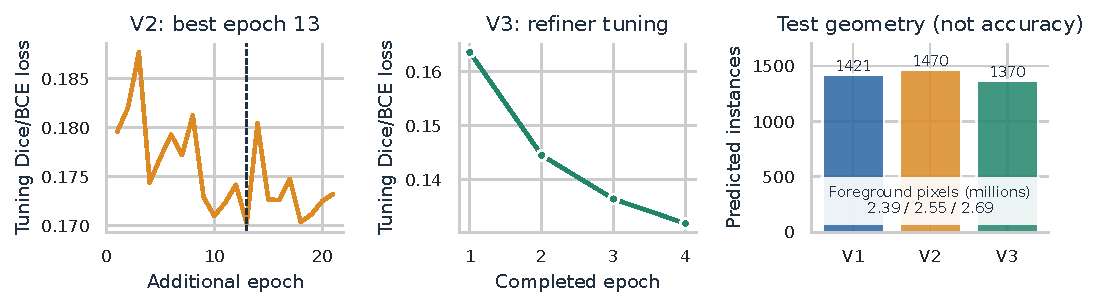
\includegraphics[width=0.75\textwidth]{figures-v2/training_and_geometry.pdf}
\caption{Saved V2/V3 training and prediction diagnostics. Prediction
geometry describes outputs, not accuracy; this panel does not depict V7.}
\label{fig:diagnostics}
\end{figure*}

\begin{figure*}[t]
\centering
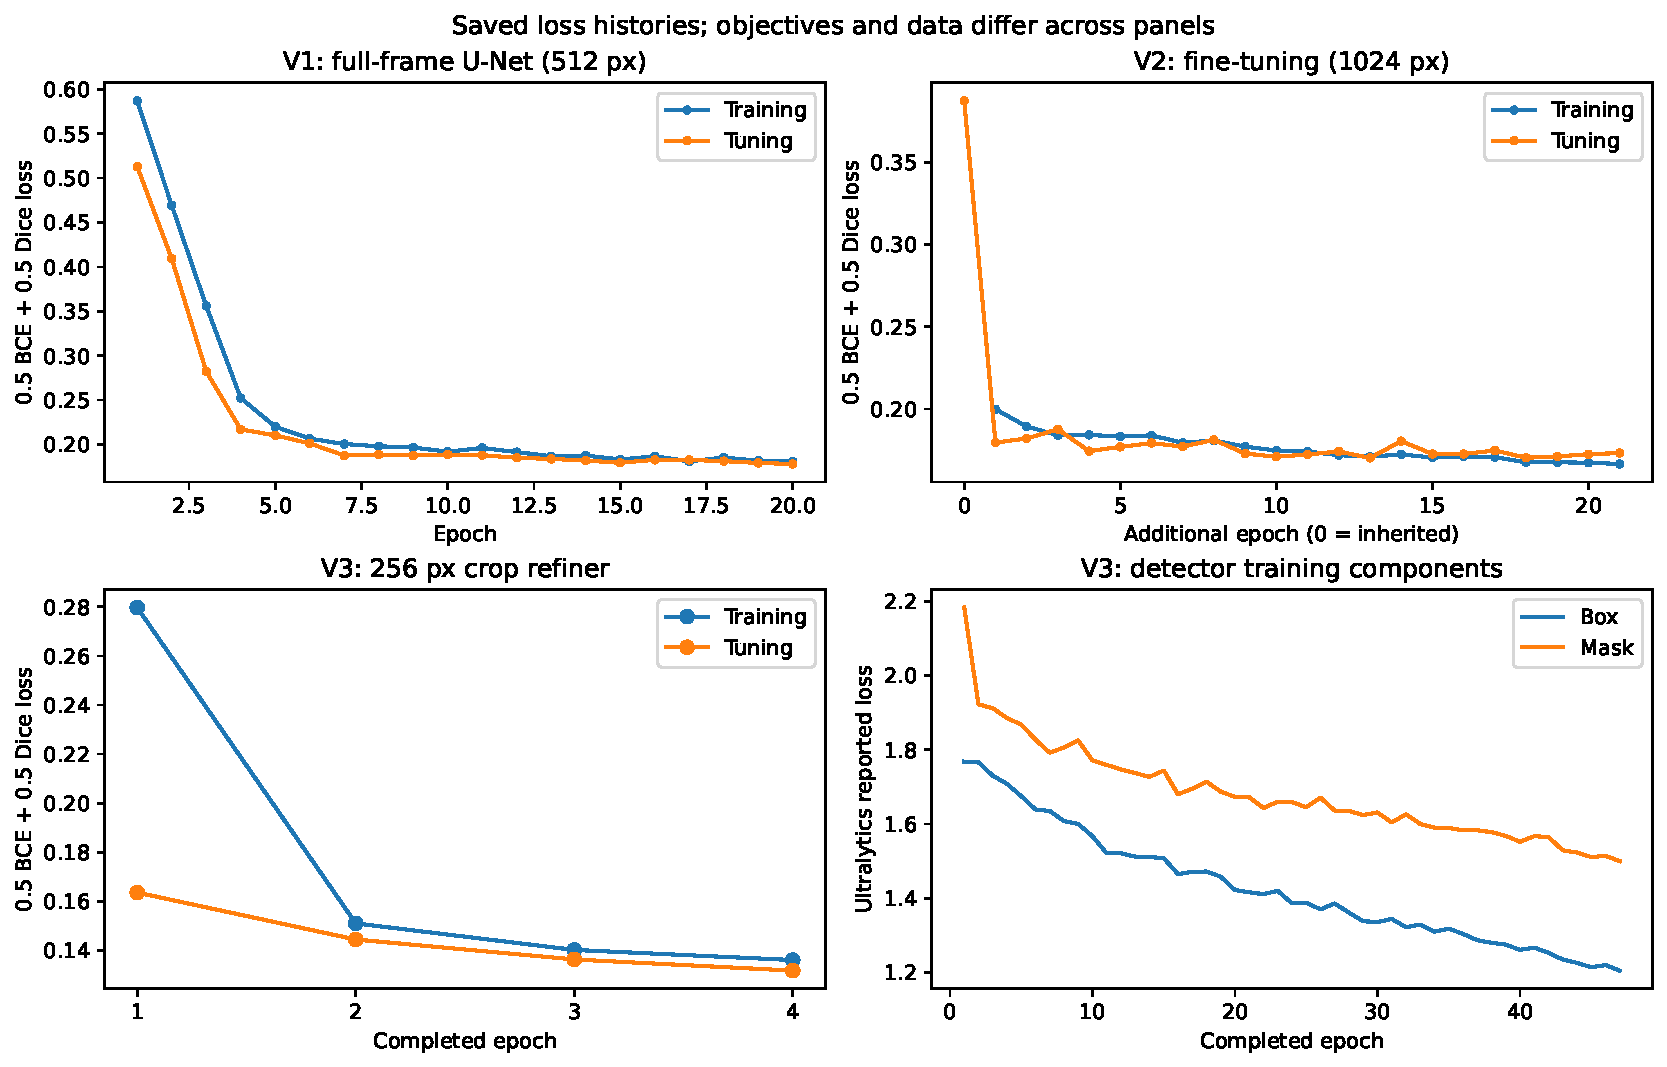
\includegraphics[width=\textwidth]{results-review/loss_by_epoch.pdf}
\caption{Saved losses by epoch. V2 epochs are additional to V1; V3's crop
refiner and detector use different objectives. Verified V5/V7 training
histories are unavailable and are not fabricated.}
\label{fig:loss}
\end{figure*}

\section{Models and Results}
\subsection{V1 and V2: Semantic Baselines}
V1 uses U-Net~\cite{unet} with an ImageNet-pretrained ResNet18
encoder~\cite{resnet}, 512-pixel input, AdamW, batch 8, 20 epochs,
and equal-weight Dice/BCE loss. Thresholding and eight-connected components
produce instances. V2 fine-tunes V1 at 1024 pixels with
CLAHE~\cite{opencvclahevisual}, batch 2, and learning rate $10^{-4}$.
It selects additional epoch 13 and stops at 21. Recorded training-stage
runtimes are 37.5 and 58.8 minutes, respectively. Submissions 58301531
and 58304132 score 0.29 and 0.32 PQ.

\subsection{V3: Proposals and Crop Refinement}
YOLO11s-seg~\cite{ultralyticsvisual} proposes instances at 1024 pixels;
a ResNet18 U-Net refines $256\times256$ crops. The detector completed
47 epochs and part of epoch 48, with a reported 1.254-hour detector run;
the refiner completed four epochs. The original CSV was rejected for
overlapping masks. Offline disjoint-mask repair without retraining produced
submission 58316663, scoring 0.35 PQ.

\subsection{V5: Five-Fold Detector/Refiner Pipeline}
Five independent YOLO11s-seg/ResNet34-U-Net pairs use day-grouped folds.
Inner tuning chooses confidence, area, and YOLO-only versus refined output;
outer labels do not select these settings~\cite{varma2006}.
Each fold trains a refiner: its output is a tuning choice, not a requirement
for every prediction. Per-fold ceilings are five detector and two refiner
epochs. Deadline-free recovery of fold 4 exceeded the two-hour target;
actual total epochs and runtime remain unavailable.

All five selected fold outputs contribute to one-to-one instance matching
at IoU at least 0.5, three-of-five instance/pixel voting, area filtering,
and disjoint ownership. Submission 58327117 scores 0.36 PQ.
Its CSV contains 1,127 masks across 177 images, with no overlaps.

\subsection{V7: YOLO-Only Follow-Up}
V7 retains five day-grouped folds and majority fusion but removes the crop
refiner. It allows up to 10 detector epochs per fold without a wall-clock
training limit, using training batch 10 across two GPUs and inference
batch 8 on GPU 0. This is a maximum of 50 detector epochs, not a verified
completed-epoch count. Submission 58336694 scores \textbf{0.26 PQ},
verified through the Kaggle API on November 14, 2026.
The exported CSV contains 2,091 disjoint masks across all 180 images.
Successful validation did not imply improved segmentation.

\section{Discussion and Conclusions}
V7's larger detector epoch allowance did not outperform the crop-capable
V3/V5 pipelines. The 0.10 PQ decrease from V5 to V7 supports prioritizing
local crop refinement in the next controlled experiment. Crops allow a
refiner to adjust proposed boundaries at a local scale, but cannot recover
objects missed by the detector. The available evidence does not establish
which V5 folds selected refinement or isolate its contribution: encoder,
training schedule, batch size, calibration, and execution also differ.

V7 predicts 964 more masks than V5 (about 86\% more). This may reflect
fragmentation, extra detections, or other grouping differences; without
test labels it cannot be equated with additional false positives.
The score decrease demonstrates that predicting more valid instances is
not sufficient.

Figure~\ref{fig:loss} shows V1 tuning loss minimized at its final epoch,
while V2 fluctuated after additional epoch 13. V3 refiner tuning loss
fell from 0.1636 to 0.1318 before its budget stop. Longer refiner training
merits testing, not a convergence claim. Losses from different objectives
and input scales are not directly comparable.

I recommend retaining the V5 pipeline as the best verified configuration
and testing matched YOLO-only/refined outputs with identical detectors,
splits, and budgets. Feature and threshold tuning should address boundaries,
missed proposals, fragmentation, and overlap ownership using labeled
validation. The conclusion is that the crop-capable pipeline performed
better here, not that cropping alone guarantees a 0.10 PQ gain.

\section{Reproducibility and Acknowledgment}
The \href{https://github.com/Greg-Kojadinovich/solar-filament-segmentation-2026}{public repository}
preserves notebooks, submissions, figures, and tests. V7's verified CSV
SHA-256 is recorded in the accompanying results manifest. Complete
reproduction still requires matching checkpoints, calibration, splits,
environments, epoch counts, and logs. The locally named ``V5 Output''
archive contains V3 artifacts and is not evidence of V5 training.

The challenge is partially supported by NSF grants 2209912, 2433781,
and 2511630, and sponsored by NSF and the National Solar Observatory.
This work uses GONG data from the NSO Integrated Synoptic Program,
operated by AURA under an NSF cooperative agreement, with NOAA
contributions. GONG is hosted by Big Bear Solar Observatory, High Altitude
Observatory, Learmonth Solar Observatory, Udaipur Solar Observatory,
Instituto de Astrofisica de Canarias, and Cerro Tololo Inter-American
Observatory.

\bibliographystyle{ACM-Reference-Format}
\bibliography{main,poster_v2,references_v3}
\end{document}
